\documentclass[]{article}
\usepackage{lmodern}
\usepackage{amssymb,amsmath}
\usepackage{ifxetex,ifluatex}
\usepackage{fixltx2e} % provides \textsubscript
\ifnum 0\ifxetex 1\fi\ifluatex 1\fi=0 % if pdftex
  \usepackage[T1]{fontenc}
  \usepackage[utf8]{inputenc}
\else % if luatex or xelatex
  \ifxetex
    \usepackage{mathspec}
  \else
    \usepackage{fontspec}
  \fi
  \defaultfontfeatures{Ligatures=TeX,Scale=MatchLowercase}
\fi
% use upquote if available, for straight quotes in verbatim environments
\IfFileExists{upquote.sty}{\usepackage{upquote}}{}
% use microtype if available
\IfFileExists{microtype.sty}{%
\usepackage{microtype}
\UseMicrotypeSet[protrusion]{basicmath} % disable protrusion for tt fonts
}{}
\usepackage[margin=1in]{geometry}
\usepackage{hyperref}
\hypersetup{unicode=true,
            pdftitle={Road Traffic Accidents Data Analysis using R},
            pdfauthor={Student ID: 201081646},
            pdfborder={0 0 0},
            breaklinks=true}
\urlstyle{same}  % don't use monospace font for urls
\usepackage{color}
\usepackage{fancyvrb}
\newcommand{\VerbBar}{|}
\newcommand{\VERB}{\Verb[commandchars=\\\{\}]}
\DefineVerbatimEnvironment{Highlighting}{Verbatim}{commandchars=\\\{\}}
% Add ',fontsize=\small' for more characters per line
\usepackage{framed}
\definecolor{shadecolor}{RGB}{248,248,248}
\newenvironment{Shaded}{\begin{snugshade}}{\end{snugshade}}
\newcommand{\KeywordTok}[1]{\textcolor[rgb]{0.13,0.29,0.53}{\textbf{{#1}}}}
\newcommand{\DataTypeTok}[1]{\textcolor[rgb]{0.13,0.29,0.53}{{#1}}}
\newcommand{\DecValTok}[1]{\textcolor[rgb]{0.00,0.00,0.81}{{#1}}}
\newcommand{\BaseNTok}[1]{\textcolor[rgb]{0.00,0.00,0.81}{{#1}}}
\newcommand{\FloatTok}[1]{\textcolor[rgb]{0.00,0.00,0.81}{{#1}}}
\newcommand{\ConstantTok}[1]{\textcolor[rgb]{0.00,0.00,0.00}{{#1}}}
\newcommand{\CharTok}[1]{\textcolor[rgb]{0.31,0.60,0.02}{{#1}}}
\newcommand{\SpecialCharTok}[1]{\textcolor[rgb]{0.00,0.00,0.00}{{#1}}}
\newcommand{\StringTok}[1]{\textcolor[rgb]{0.31,0.60,0.02}{{#1}}}
\newcommand{\VerbatimStringTok}[1]{\textcolor[rgb]{0.31,0.60,0.02}{{#1}}}
\newcommand{\SpecialStringTok}[1]{\textcolor[rgb]{0.31,0.60,0.02}{{#1}}}
\newcommand{\ImportTok}[1]{{#1}}
\newcommand{\CommentTok}[1]{\textcolor[rgb]{0.56,0.35,0.01}{\textit{{#1}}}}
\newcommand{\DocumentationTok}[1]{\textcolor[rgb]{0.56,0.35,0.01}{\textbf{\textit{{#1}}}}}
\newcommand{\AnnotationTok}[1]{\textcolor[rgb]{0.56,0.35,0.01}{\textbf{\textit{{#1}}}}}
\newcommand{\CommentVarTok}[1]{\textcolor[rgb]{0.56,0.35,0.01}{\textbf{\textit{{#1}}}}}
\newcommand{\OtherTok}[1]{\textcolor[rgb]{0.56,0.35,0.01}{{#1}}}
\newcommand{\FunctionTok}[1]{\textcolor[rgb]{0.00,0.00,0.00}{{#1}}}
\newcommand{\VariableTok}[1]{\textcolor[rgb]{0.00,0.00,0.00}{{#1}}}
\newcommand{\ControlFlowTok}[1]{\textcolor[rgb]{0.13,0.29,0.53}{\textbf{{#1}}}}
\newcommand{\OperatorTok}[1]{\textcolor[rgb]{0.81,0.36,0.00}{\textbf{{#1}}}}
\newcommand{\BuiltInTok}[1]{{#1}}
\newcommand{\ExtensionTok}[1]{{#1}}
\newcommand{\PreprocessorTok}[1]{\textcolor[rgb]{0.56,0.35,0.01}{\textit{{#1}}}}
\newcommand{\AttributeTok}[1]{\textcolor[rgb]{0.77,0.63,0.00}{{#1}}}
\newcommand{\RegionMarkerTok}[1]{{#1}}
\newcommand{\InformationTok}[1]{\textcolor[rgb]{0.56,0.35,0.01}{\textbf{\textit{{#1}}}}}
\newcommand{\WarningTok}[1]{\textcolor[rgb]{0.56,0.35,0.01}{\textbf{\textit{{#1}}}}}
\newcommand{\AlertTok}[1]{\textcolor[rgb]{0.94,0.16,0.16}{{#1}}}
\newcommand{\ErrorTok}[1]{\textcolor[rgb]{0.64,0.00,0.00}{\textbf{{#1}}}}
\newcommand{\NormalTok}[1]{{#1}}
\usepackage{graphicx,grffile}
\makeatletter
\def\maxwidth{\ifdim\Gin@nat@width>\linewidth\linewidth\else\Gin@nat@width\fi}
\def\maxheight{\ifdim\Gin@nat@height>\textheight\textheight\else\Gin@nat@height\fi}
\makeatother
% Scale images if necessary, so that they will not overflow the page
% margins by default, and it is still possible to overwrite the defaults
% using explicit options in \includegraphics[width, height, ...]{}
\setkeys{Gin}{width=\maxwidth,height=\maxheight,keepaspectratio}
\IfFileExists{parskip.sty}{%
\usepackage{parskip}
}{% else
\setlength{\parindent}{0pt}
\setlength{\parskip}{6pt plus 2pt minus 1pt}
}
\setlength{\emergencystretch}{3em}  % prevent overfull lines
\providecommand{\tightlist}{%
  \setlength{\itemsep}{0pt}\setlength{\parskip}{0pt}}
\setcounter{secnumdepth}{5}
% Redefines (sub)paragraphs to behave more like sections
\ifx\paragraph\undefined\else
\let\oldparagraph\paragraph
\renewcommand{\paragraph}[1]{\oldparagraph{#1}\mbox{}}
\fi
\ifx\subparagraph\undefined\else
\let\oldsubparagraph\subparagraph
\renewcommand{\subparagraph}[1]{\oldsubparagraph{#1}\mbox{}}
\fi

%%% Use protect on footnotes to avoid problems with footnotes in titles
\let\rmarkdownfootnote\footnote%
\def\footnote{\protect\rmarkdownfootnote}

%%% Change title format to be more compact
\usepackage{titling}

% Create subtitle command for use in maketitle
\newcommand{\subtitle}[1]{
  \posttitle{
    \begin{center}\large#1\end{center}
    }
}

\setlength{\droptitle}{-2em}

  \title{Road Traffic Accidents Data Analysis using R}
    \pretitle{\vspace{\droptitle}\centering\huge}
  \posttitle{\par}
    \author{Student ID: 201081646}
    \preauthor{\centering\large\emph}
  \postauthor{\par}
    \date{}
    \predate{}\postdate{}
  
\usepackage{float} \floatplacement{figure}{H}

\begin{document}
\maketitle

\section{Introduction}\label{introduction}

This report is the second assessment of the \textbf{MATH5741M
Statistical Theory and Methods} module. Its aim is to analyse a road
traffic accidents dataset collected by the UK Department for Transport
(DfT) in 2005 trough different statistical methods such as boxplot
visualisations, statistical hypothesis testing, and confidence
intervals.

It has been done using \textbf{R} (programming language) and it is code
reproducible. To see the whole code written for its performance visit
\url{https://github.com/eugenividal/Road-Traffic-Accidents-Data-Analysis}

\section{Data preparation}\label{data-preparation}

First, we activate the libraries we will need to set up the project.

\begin{Shaded}
\begin{Highlighting}[]
\CommentTok{# Activate libraries}
\KeywordTok{library}\NormalTok{(tidyverse)}
\KeywordTok{library}\NormalTok{(cowplot)}
\end{Highlighting}
\end{Shaded}

Second, we load the data into the \textbf{R} environment.

\begin{Shaded}
\begin{Highlighting}[]
\CommentTok{# Read csv in R}
\CommentTok{#xx=read.csv("http://www1.maths.leeds.ac.uk/~charles/math5741/DfTaccidents.csv", header =T)}
\NormalTok{xx=}\KeywordTok{read.csv}\NormalTok{(}\StringTok{"DfTaccidents.csv"}\NormalTok{, }\DataTypeTok{header=}\NormalTok{T)}
\end{Highlighting}
\end{Shaded}

The next step is to drop all those columns we will not need to perform
our analysis. We only need: number of vehicles, type of area and day of
the week.

Then, we transform the variables

\begin{Shaded}
\begin{Highlighting}[]
\CommentTok{# Rename labels of Urban_or_Rural_Area}
\NormalTok{xx$Urban_or_Rural_Area[xx$Urban_or_Rural_Area ==}\StringTok{ "1"}\NormalTok{] <-}\StringTok{ "Urban"}
\NormalTok{xx$Urban_or_Rural_Area[xx$Urban_or_Rural_Area ==}\StringTok{ "2"}\NormalTok{] <-}\StringTok{ "Rural"}
\NormalTok{xx$Urban_or_Rural_Area[xx$Urban_or_Rural_Area ==}\StringTok{ "3"}\NormalTok{] <-}\StringTok{ "Unallocated"}

\CommentTok{# Rename labels of day of the week}
\NormalTok{xx$Day_of_Week[xx$Day_of_Week ==}\StringTok{ "1"}\NormalTok{] <-}\StringTok{ "Sunday"}
\NormalTok{xx$Day_of_Week[xx$Day_of_Week ==}\StringTok{ "2"}\NormalTok{] <-}\StringTok{ "Monday"}
\NormalTok{xx$Day_of_Week[xx$Day_of_Week ==}\StringTok{ "3"}\NormalTok{] <-}\StringTok{ "Tuesday"}
\NormalTok{xx$Day_of_Week[xx$Day_of_Week ==}\StringTok{ "4"}\NormalTok{] <-}\StringTok{ "Wednesday"}
\NormalTok{xx$Day_of_Week[xx$Day_of_Week ==}\StringTok{ "5"}\NormalTok{] <-}\StringTok{ "Thursday"}
\NormalTok{xx$Day_of_Week[xx$Day_of_Week ==}\StringTok{ "6"}\NormalTok{] <-}\StringTok{ "Friday"}
\NormalTok{xx$Day_of_Week[xx$Day_of_Week ==}\StringTok{ "7"}\NormalTok{] <-}\StringTok{ "Saturday"}

\CommentTok{#xx$Day_of_Week  <- factor(xx$Day_of_Week , levels= c("Sunday", "Monday", }
\CommentTok{#    "Tuesday", "Wednesday", "Thursday", "Friday", "Saturday"))}
\end{Highlighting}
\end{Shaded}

Finally, we show the the dataset ready for exploration.

\begin{Shaded}
\begin{Highlighting}[]
\CommentTok{# Show first 6 rows}
\KeywordTok{head}\NormalTok{(xx)}
\end{Highlighting}
\end{Shaded}

\begin{verbatim}
##   Number_of_Vehicles Day_of_Week Urban_or_Rural_Area
## 1                  1     Tuesday               Urban
## 2                  1   Wednesday               Urban
## 3                  2    Thursday               Urban
## 4                  1      Friday               Urban
## 5                  1      Monday               Urban
## 6                  2     Tuesday               Urban
\end{verbatim}

\section{Data exploration}\label{data-exploration}

\subsection{Boxplot}\label{boxplot}

To compare the number of vehicles involved in urban areas with the
number involved in a rural areas, we plot a boxplot. However, the graph
is not very clear. To check what might be the problem, we plot a
histogram. The data is not symetric, it is very skewed to the left (see
histogram 1). To normalise it, I first plot three different
transformations: log2, log10 and sqrt. Then, I chose log10 to plot the
boxplot again.

\begin{center}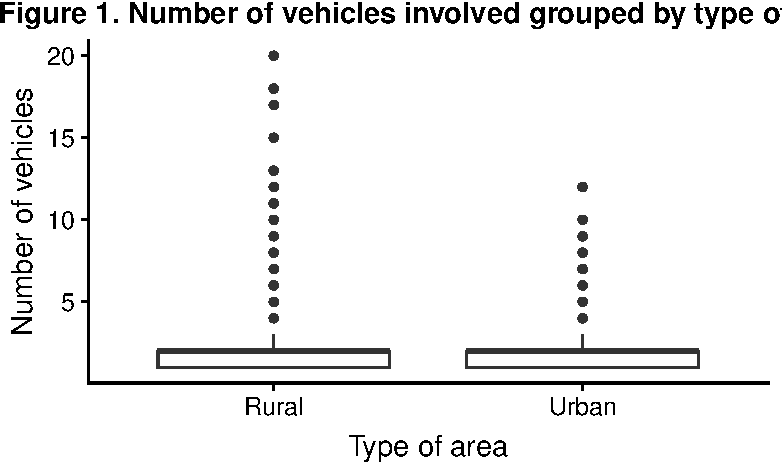
\includegraphics{README_files/figure-latex/unnamed-chunk-7-1} \end{center}

\begin{verbatim}
##    Min. 1st Qu.  Median    Mean 3rd Qu.    Max. 
##   1.000   1.000   2.000   1.843   2.000  20.000
\end{verbatim}

\begin{verbatim}
##    Min. 1st Qu.  Median    Mean 3rd Qu.    Max. 
##  0.0000  0.0000  1.0000  0.7761  1.0000  4.3219
\end{verbatim}

\begin{verbatim}
##    Min. 1st Qu.  Median    Mean 3rd Qu.    Max. 
##  0.0000  0.0000  0.3010  0.2336  0.3010  1.3010
\end{verbatim}

\begin{verbatim}
##    Min. 1st Qu.  Median    Mean 3rd Qu.    Max. 
##   1.000   1.000   1.414   1.333   1.414   4.472
\end{verbatim}

\begin{center}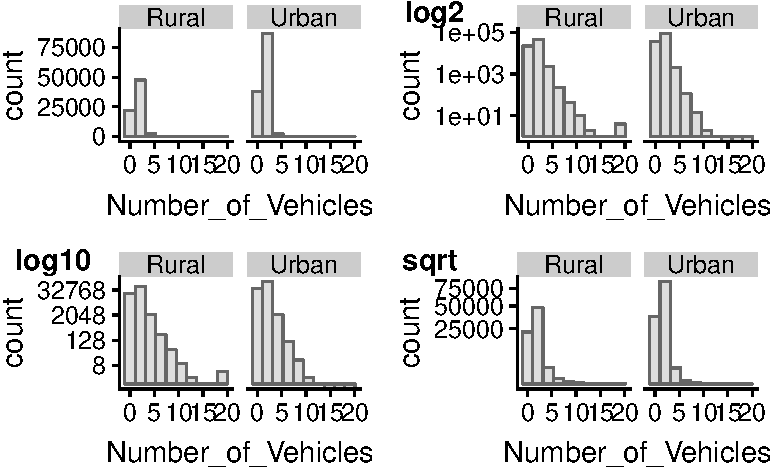
\includegraphics{README_files/figure-latex/unnamed-chunk-7-2} \end{center}

\begin{center}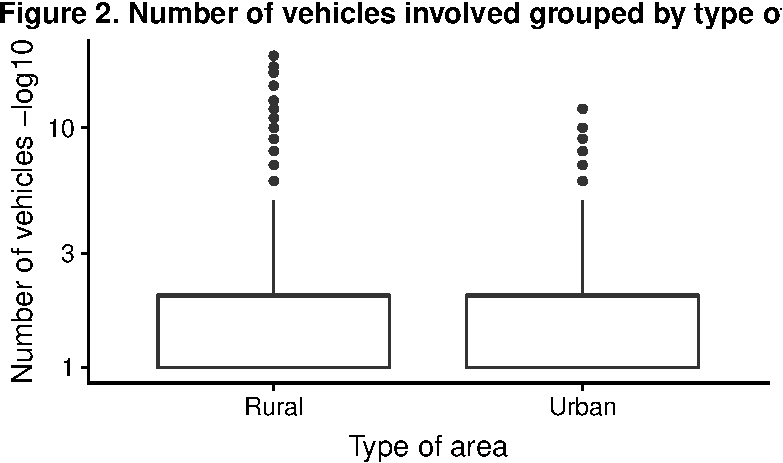
\includegraphics{README_files/figure-latex/unnamed-chunk-7-3} \end{center}

However, from the boxplot we can not whether the average number of
vehicles in an accident differ in urban and rural areas. To do this, we
perform a test.

?chisq.test

This is the same as exercise C4 too.

\url{https://statistics.laerd.com/statistical-guides/independent-t-test-statistical-guide.php}

These are two-tailed tests of population mean with unknown variance.
Pooled variance test?

\[H_{0}: \mu_{u} = \mu_{r}\;\;\;vs.\;\;\;H_{1}: \mu_{u} \neq \mu_{r}\]

\begin{Shaded}
\begin{Highlighting}[]
\CommentTok{# Check the variance of the two groups}
\NormalTok{xx_area$log10 <-}\StringTok{ }\KeywordTok{log10}\NormalTok{(xx_area$Number_of_Vehicles)}
\NormalTok{Urban_or_Rural_Area <-}\StringTok{ }\NormalTok{xx_area$Urban_or_Rural_Area}
\KeywordTok{var}\NormalTok{(xx_area[Urban_or_Rural_Area==}\StringTok{"Urban"}\NormalTok{,}\DecValTok{4}\NormalTok{])        }\CommentTok{# apply the var function }
\end{Highlighting}
\end{Shaded}

\begin{verbatim}
## [1] 0.02632199
\end{verbatim}

\begin{Shaded}
\begin{Highlighting}[]
\KeywordTok{var}\NormalTok{(xx_area[Urban_or_Rural_Area==}\StringTok{"Rural"}\NormalTok{,}\DecValTok{4}\NormalTok{])}
\end{Highlighting}
\end{Shaded}

\begin{verbatim}
## [1] 0.03153835
\end{verbatim}

They are not about the same, should we continue with a two sample test
which assumes equal variance? The independent t-test assumes the
variances of the two groups you are measuring are equal in the
population. If your variances are unequal, this can affect the Type I
error rate. The assumption of homogeneity of variance can be tested
using Levene's Test of Equality of Variances.

\begin{Shaded}
\begin{Highlighting}[]
\CommentTok{# pooled variance test}
\CommentTok{#t.test(xx[])}
\end{Highlighting}
\end{Shaded}

In conclusion, we can say that

\subsection{Statistical hypothesis}\label{statistical-hypothesis}

Comparing frequency counts between two groups of different sample.

Chi-squared test?

In this section, we investigate whether the frequency of accidents
varies by day of the week. To do this we use a statistical hypotesis
test.

*Note that here the unallocated accidents are included.

\begin{Shaded}
\begin{Highlighting}[]
\CommentTok{# hypothesis per each day}
\KeywordTok{ggplot}\NormalTok{(xx, }\KeywordTok{aes}\NormalTok{(}\DataTypeTok{x=}\NormalTok{Day_of_Week))+}\KeywordTok{geom_bar}\NormalTok{() +}
\StringTok{  }\KeywordTok{theme}\NormalTok{(}\DataTypeTok{axis.text.x =} \KeywordTok{element_text}\NormalTok{(}\DataTypeTok{angle =} \DecValTok{45}\NormalTok{, }\DataTypeTok{hjust=}\DecValTok{1}\NormalTok{))}
\end{Highlighting}
\end{Shaded}

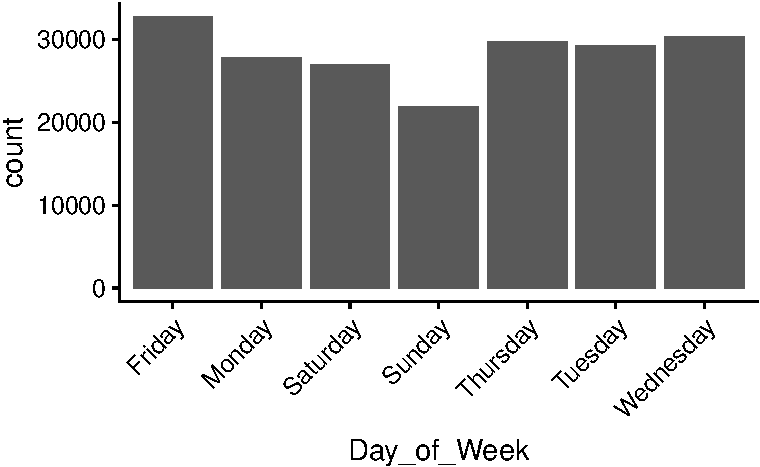
\includegraphics{README_files/figure-latex/unnamed-chunk-10-1.pdf}

Next, we are asked to do the same test using only week-days (excluding
Saturday and Sunday).

\begin{Shaded}
\begin{Highlighting}[]
\CommentTok{# Select data using only week-days}
\NormalTok{week_days <-}\StringTok{ }\NormalTok{xx%>%}
\StringTok{  }\KeywordTok{select}\NormalTok{(Day_of_Week)%>%}
\StringTok{  }\KeywordTok{filter}\NormalTok{(!Day_of_Week %in%}\StringTok{ }\KeywordTok{c}\NormalTok{(}\StringTok{"Saturday"}\NormalTok{, }\StringTok{"Sunday"}\NormalTok{))}
\end{Highlighting}
\end{Shaded}

\begin{verbatim}
## Warning: package 'bindrcpp' was built under R version 3.4.4
\end{verbatim}

\begin{Shaded}
\begin{Highlighting}[]
\KeywordTok{table}\NormalTok{(week_days)}
\end{Highlighting}
\end{Shaded}

\begin{verbatim}
## week_days
##    Friday    Monday  Thursday   Tuesday Wednesday 
##     32738     27812     29738     29219     30373
\end{verbatim}

\begin{Shaded}
\begin{Highlighting}[]
\KeywordTok{ggplot}\NormalTok{(week_days, }\KeywordTok{aes}\NormalTok{(}\DataTypeTok{x=}\NormalTok{Day_of_Week))+}\KeywordTok{geom_bar}\NormalTok{() +}
\StringTok{  }\KeywordTok{theme}\NormalTok{(}\DataTypeTok{axis.text.x =} \KeywordTok{element_text}\NormalTok{(}\DataTypeTok{angle =} \DecValTok{45}\NormalTok{, }\DataTypeTok{hjust=}\DecValTok{1}\NormalTok{)) }
\end{Highlighting}
\end{Shaded}

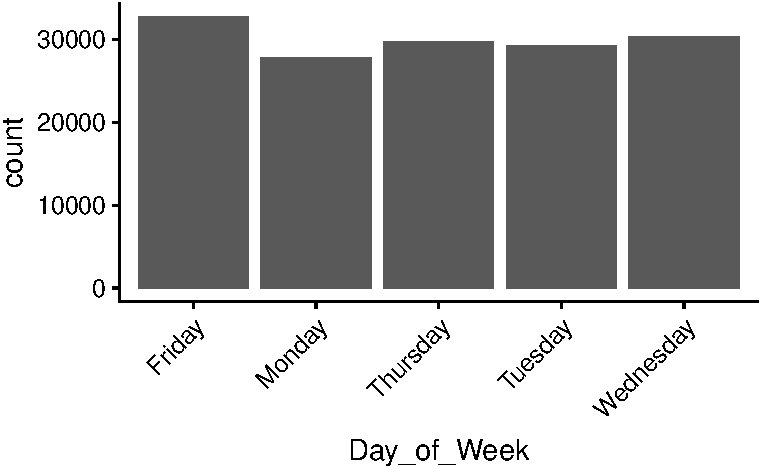
\includegraphics{README_files/figure-latex/unnamed-chunk-11-1.pdf}

\begin{Shaded}
\begin{Highlighting}[]
\CommentTok{# hypothesis per each day using only week-days}
\end{Highlighting}
\end{Shaded}

\subsection{Confidence interval}\label{confidence-interval}

Finally, in this section, we compute a 95\% confidence interval for the
expected (mean) number of accidents which occur on a Monday.

\begin{Shaded}
\begin{Highlighting}[]
\CommentTok{# Select data using only week-days}
\NormalTok{week_days<-}\StringTok{ }\NormalTok{xx%>%}
\StringTok{  }\KeywordTok{select}\NormalTok{(Day_of_Week)%>%}
\StringTok{  }\KeywordTok{filter}\NormalTok{(Day_of_Week ==}\StringTok{ "Monday"}\NormalTok{)}
\end{Highlighting}
\end{Shaded}

\subsection{Bibliography}\label{bibliography}

The resources used to carry out this project are:

\begin{itemize}
\tightlist
\item
  Balka, J. 2013. JBStatistics: Making Statistics Make Sense. Available
  from: \url{http://www.jbstatistics.com}.
\item
  Lane, D.M. 2018. Online Statistics Education: An Interactive
  Multimedia Course of Study. Available from:
  \url{http://onlinestatbook.com/}.
\item
  Taylor, C. 2017. MATH5741M: Statistical Theory and Methods. Outline
  Lecture Notes.
\item
  Yau, C. 2018. R tutorial: an R introduction to statistics. Available
  from: \url{http://www.r-tutor.com}
\end{itemize}


\end{document}
